\documentclass[usepdftitle=false,hyperref={pdfpagelabels=false}]{beamer}

% use KIT-Theme
% see http://sdqweb.ipd.kit.edu/wiki/Dokumentvorlagen
%\usetheme{Frankfurt} % see http://deic.uab.es/~iblanes/beamer_gallery/index_by_theme.html
\InputIfFileExists{templates/beamerthemekit.sty}{\usepackage{templates/beamerthemekit}}{\usetheme{Frankfurt}}
\usefonttheme{professionalfonts}


\usepackage{hyperref}
\usepackage{lmodern}
\usepackage{listings}
\usepackage{wrapfig}        % see http://en.wikibooks.org/wiki/LaTeX/Floats,_Figures_and_Captions

\usepackage[utf8]{inputenc} % this is needed for german umlauts
\usepackage[ngerman]{babel} % this is needed for german umlauts
\usepackage[T1]{fontenc}    % this is needed for correct output of umlauts in pdf

\usepackage{verbatim}
\usepackage{relsize}
\usepackage{subfigure}

% http://en.wikibooks.org/wiki/LaTeX/Algorithms_and_Pseudocode
% http://tex.stackexchange.com/questions/1375/what-is-a-good-package-for-displaying-algorithms
% http://tex.stackexchange.com/questions/26539/beamer-and-pseudocode
% http://www.jkrieger.de/tools/latex/informatik.html
% http://ctan.mackichan.com/macros/latex/contrib/algorithmicx/algorithmicx.pdf
% http://ctan.mackichan.com/macros/latex/contrib/algorithms/algorithms.pdf
% http://www.cs.brown.edu/system/software/latex/doc/algodoc.pdf
% http://www.cs.utexas.edu/~shan/doc/algorithms.pdf
\usepackage{algorithm,algpseudocode}
\usepackage{tikz}
\usetikzlibrary{arrows,shapes,positioning,shadows,calc}
\usepackage{tkz-berge}
\usepackage{xcolor}
\makeatletter

% to change colors
\newcommand{\fillcol}{green!20}
\newcommand{\bordercol}{black}

%%%%%%%%%%%%%%%%%%%%%%%%%%%%%%%%%%%%%%%%%%%%%%%%%%%%%%%%%%%%%%%%%%%%%%
%%%%%%%%%%%%%%%%%%%%%%%%%%%%%%%%%%%%%%%%%%%%%%%%%%%%%%%%%%%%%%%%%%%%%%
% code from Andrew Stacey (with small adjustment to the border color)
% http://tex.stackexchange.com/questions/51582/background-coloring-with-overlay-specification-in-algorithm2e-beamer-package
\newcounter{jumping}
\resetcounteronoverlays{jumping}

\def\jump@setbb#1#2#3{%
  \@ifundefined{jump@#1@maxbb}{%
    \expandafter\gdef\csname jump@#1@maxbb\endcsname{#3}%
  }{%
    \csname jump@#1@maxbb\endcsname
    \pgf@xa=\pgf@x
    \pgf@ya=\pgf@y
    #3
    \pgfmathsetlength\pgf@x{max(\pgf@x,\pgf@xa)}%
    \pgfmathsetlength\pgf@y{max(\pgf@y,\pgf@ya)}%
    \expandafter\xdef\csname jump@#1@maxbb\endcsname{\noexpand\pgfpoint{\the\pgf@x}{\the\pgf@y}}%
  }
  \@ifundefined{jump@#1@minbb}{%
    \expandafter\gdef\csname jump@#1@minbb\endcsname{#2}%
  }{%
    \csname jump@#1@minbb\endcsname
    \pgf@xa=\pgf@x
    \pgf@ya=\pgf@y
    #2
    \pgfmathsetlength\pgf@x{min(\pgf@x,\pgf@xa)}%
    \pgfmathsetlength\pgf@y{min(\pgf@y,\pgf@ya)}%
    \expandafter\xdef\csname jump@#1@minbb\endcsname{\noexpand\pgfpoint{\the\pgf@x}{\the\pgf@y}}%
  }
}

\tikzset{%
  remember picture with id/.style={%
    remember picture,
    overlay,
    draw=\bordercol,
    save picture id=#1,
  },
  save picture id/.code={%
    \edef\pgf@temp{#1}%
    \immediate\write\pgfutil@auxout{%
      \noexpand\savepointas{\pgf@temp}{\pgfpictureid}}%
  },
  if picture id/.code args={#1#2#3}{%
    \@ifundefined{save@pt@#1}{%
      \pgfkeysalso{#3}%
    }{
      \pgfkeysalso{#2}%
    }
  },
  onslide/.code args={<#1>#2}{%
    \only<#1>{\pgfkeysalso{#2}}%
  },
  alt/.code args={<#1>#2#3}{%
    \alt<#1>{\pgfkeysalso{#2}}{\pgfkeysalso{#3}}%
  },
  stop jumping/.style={
    execute at end picture={%
      \stepcounter{jumping}%
      \immediate\write\pgfutil@auxout{%
        \noexpand\jump@setbb{\the\value{jumping}}{\noexpand\pgfpoint{\the\pgf@picminx}{\the\pgf@picminy}}{\noexpand\pgfpoint{\the\pgf@picmaxx}{\the\pgf@picmaxy}}
      },
      \csname jump@\the\value{jumping}@maxbb\endcsname
      \path (\the\pgf@x,\the\pgf@y);
      \csname jump@\the\value{jumping}@minbb\endcsname
      \path (\the\pgf@x,\the\pgf@y);
    },
  }
}


\def\savepointas#1#2{%
  \expandafter\gdef\csname save@pt@#1\endcsname{#2}%
}

\def\tmk@labeldef#1,#2\@nil{%
  \def\tmk@label{#1}%
  \def\tmk@def{#2}%
}

\tikzdeclarecoordinatesystem{pic}{%
  \pgfutil@in@,{#1}%
  \ifpgfutil@in@%
    \tmk@labeldef#1\@nil
  \else
    \tmk@labeldef#1,\pgfpointorigin\@nil
  \fi
  \@ifundefined{save@pt@\tmk@label}{%
    \tikz@scan@one@point\pgfutil@firstofone\tmk@def
  }{%
  \pgfsys@getposition{\csname save@pt@\tmk@label\endcsname}\save@orig@pic%
  \pgfsys@getposition{\pgfpictureid}\save@this@pic%
  \pgf@process{\pgfpointorigin\save@this@pic}%
  \pgf@xa=\pgf@x
  \pgf@ya=\pgf@y
  \pgf@process{\pgfpointorigin\save@orig@pic}%
  \advance\pgf@x by -\pgf@xa
  \advance\pgf@y by -\pgf@ya
  }%
}
\newcommand\tikzmark[2][]{%
\tikz[remember picture with id=#2] #1;}
\makeatother

\resetcounteronoverlays{algocf}

\newcommand<>{\boxto}[1]{%
\only#2{\tikz[remember picture with id=#1]
\draw[line width=1pt,fill=\fillcol,rectangle,rounded corners]
(pic cs:#1) ++(5.2,-.1) rectangle (-0.4,0)
;\tikz\node [anchor=base] (#1){};}% <= insertion to store the anchor to be used as based for the annotation
}
%%%%%%%%%%%%%%%%%%%%%%%%%%%%%%%%%%%%%%%%%%%%%%%%%%%%%%%%%%%%%%%%%%%%%%
%%%%%%%%%%%%%%%%%%%%%%%%%%%%%%%%%%%%%%%%%%%%%%%%%%%%%%%%%%%%%%%%%%%%%%

% Define some styles for graphs
\tikzstyle{vertex}=[circle,fill=black!25,minimum size=20pt,inner sep=0pt]
\tikzstyle{selected vertex} = [vertex, fill=red!24]
\tikzstyle{blue vertex} = [vertex, fill=blue!24]
\tikzstyle{yellow vertex} = [vertex, fill=yellow!24]
\tikzstyle{edge} = [draw,thick,-]
\tikzstyle{weight} = [font=\small]
\tikzstyle{selected edge} = [draw,line width=5pt,-,red!50]
\tikzstyle{ignored edge} = [draw,line width=5pt,-,black!20]

\hypersetup{pdftitle={Graphentheorie II}}
\beamertemplatenavigationsymbolsempty

\newcommand\InsertToC[1][]{
  \begin{frame}{Outline}
    \tableofcontents[subsectionstyle=show/show/show, subsubsectionstyle=show/show/show, #1]
  \end{frame}
}

\begin{document}
\title{Graphentheorie II}
\author{Tobias Sturm, Martin Thoma, Max Wagner, Thomas Krings}
\date{\today}
\subject{Graphentheorie-Referat fur ICPC}

\frame{\titlepage}

\frame{
	\frametitle{Inhaltsverzeichnis}
	\setcounter{tocdepth}{1}
	\tableofcontents
	\setcounter{tocdepth}{2}
}

\AtBeginSection[]{
	\InsertToC[sections={\thesection}]  % shows only subsubsections of one subsection
}

\section{Minimale Spannbäume}

\subsection{Wozu minimale Spannbäume?}
\begin{frame}{Wozu?}{Why?}
	\only<1>{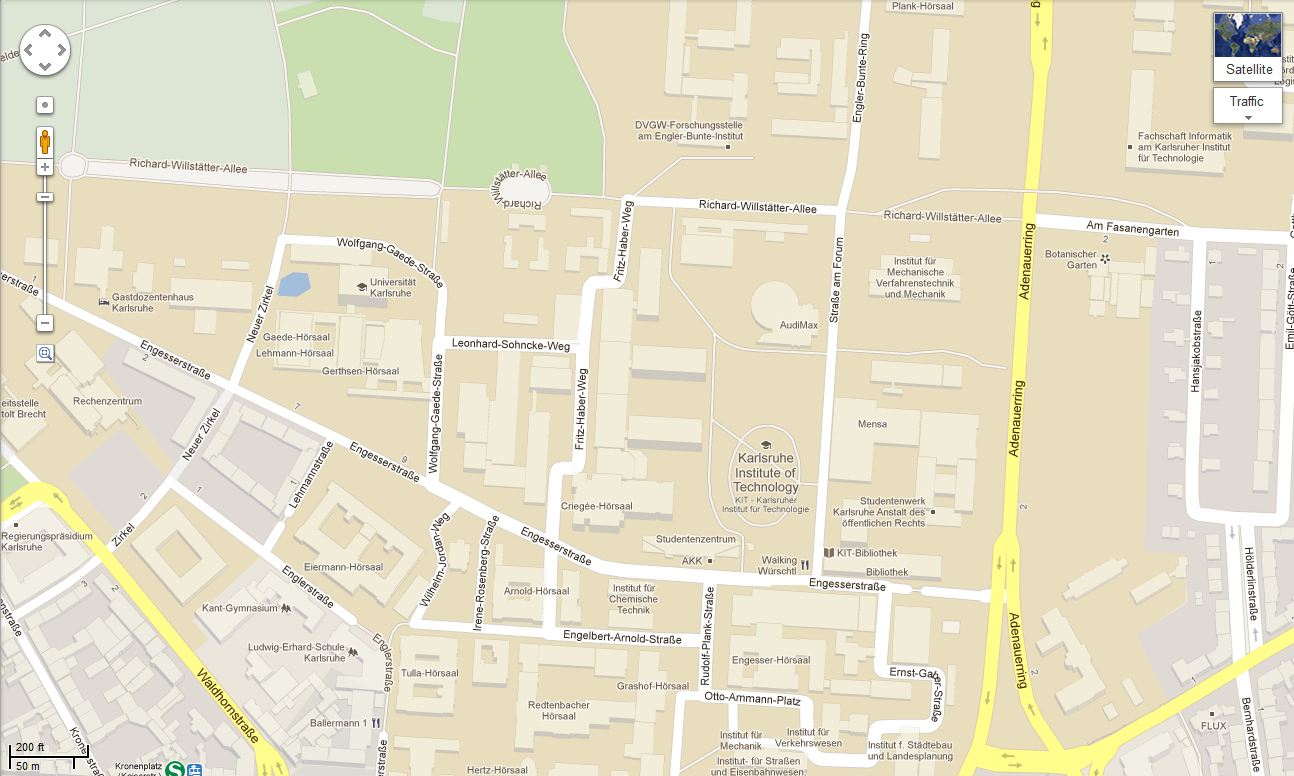
\includegraphics[scale=0.35]{Material/minSpannbaum_1.png}}
	\only<2>{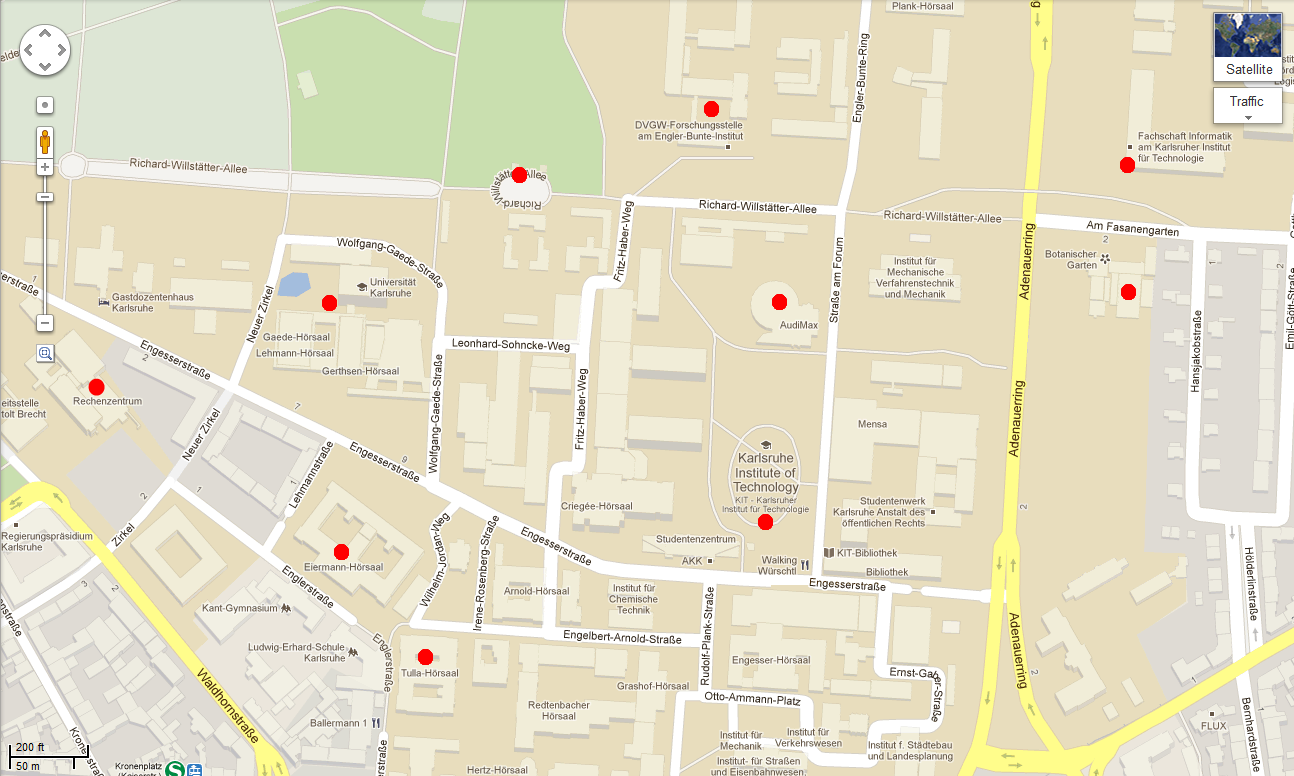
\includegraphics[scale=0.35]{Material/minSpannbaum_2.png}}
	\only<3>{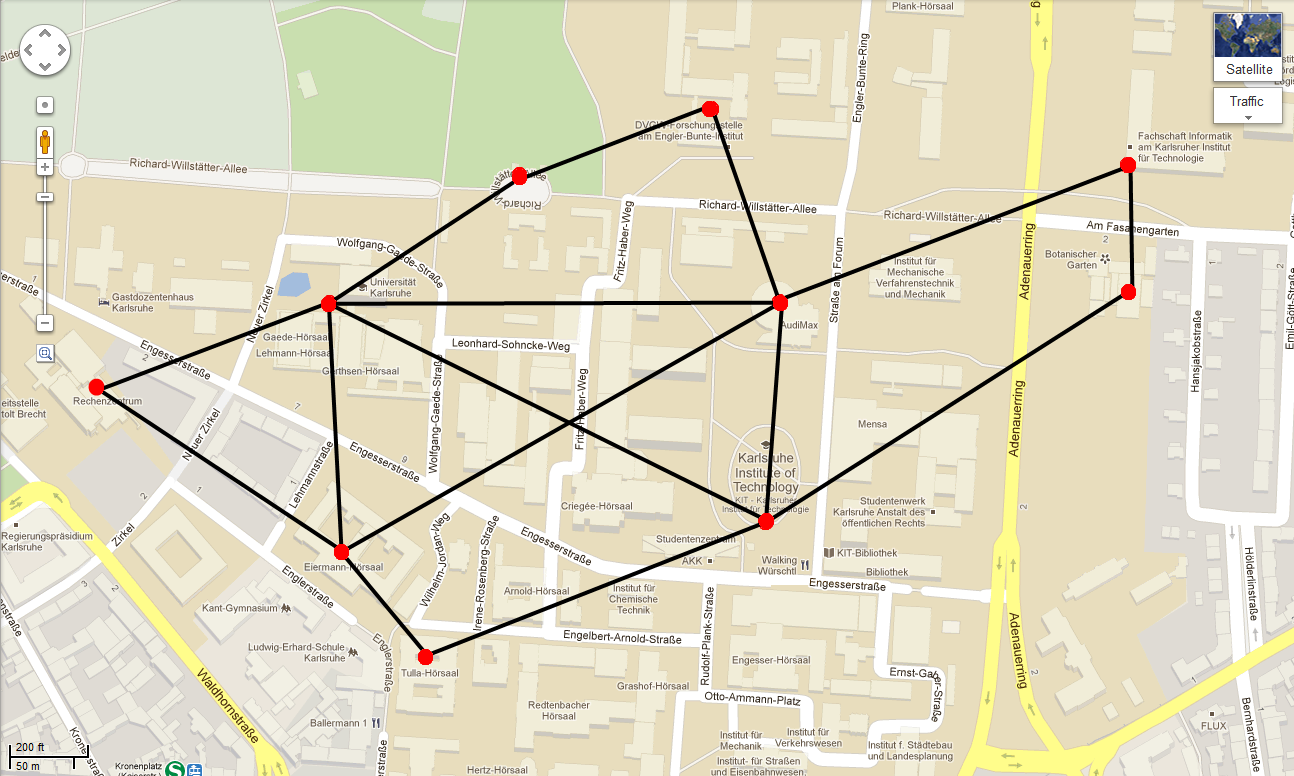
\includegraphics[scale=0.35]{Material/minSpannbaum_3.png}}
	\only<4>{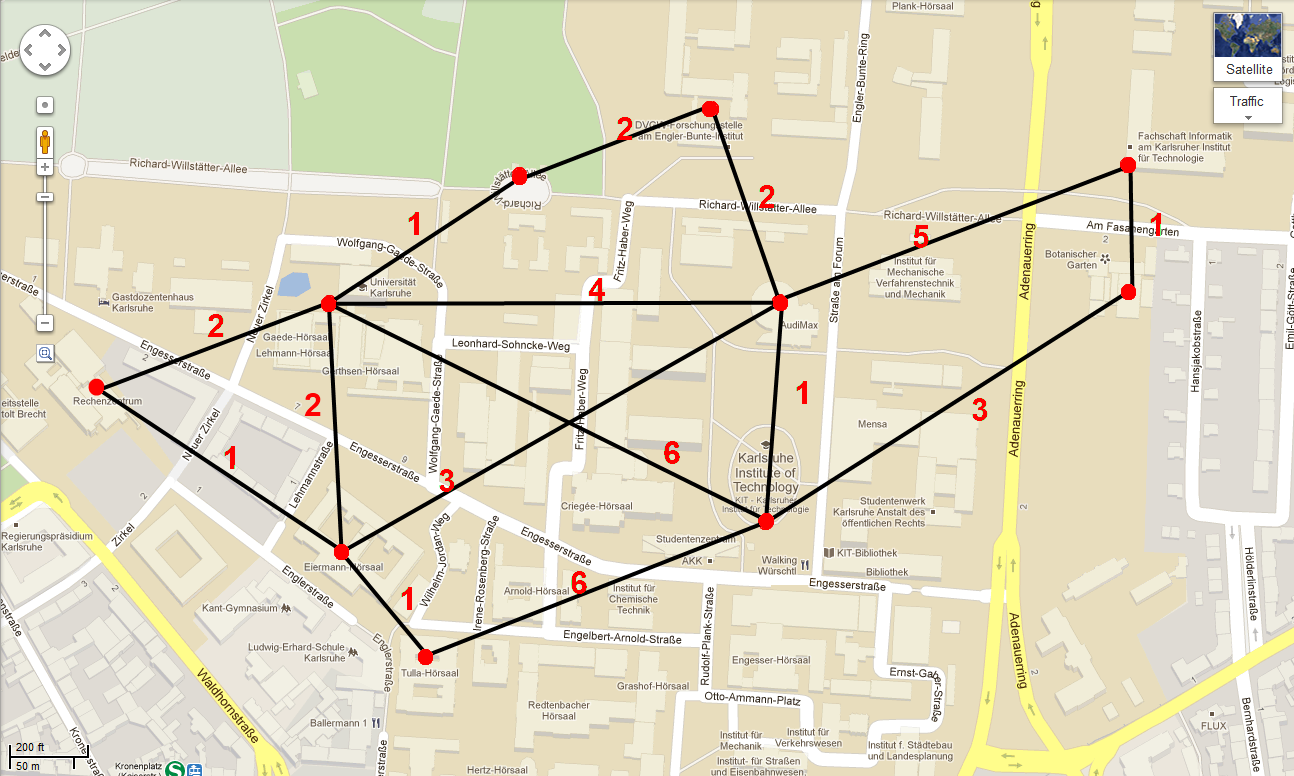
\includegraphics[scale=0.35]{Material/minSpannbaum_4.png}}
	\only<5>{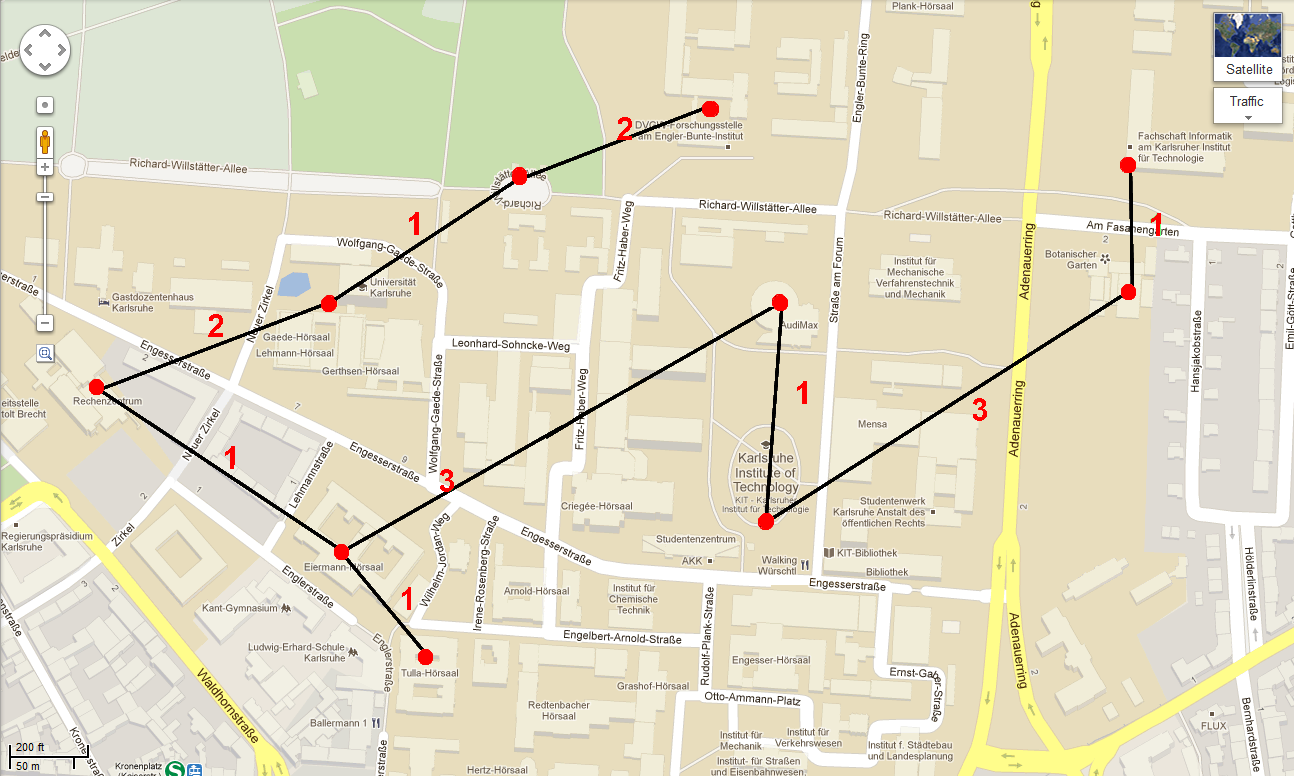
\includegraphics[scale=0.35]{Material/minSpannbaum_5.png}}
\end{frame}

\subsection{Was ist ein minimaler Spannbaum?}
\begin{frame}{Definition}
Minimale Spannbäume sind Teilgraphen, sodass ...
	\begin{itemize}
		\item ... alle Knoten erreichbar sind \pause
		\item ... die Summe der Kantengewichte minimal ist \pause
		\item ... kein Zyklus im Graph enthalten ist ($\Rightarrow$ Baum).
	\end{itemize}
\end{frame}

\begin{frame}{Definition}
	Sei	$G = (V, E) $ mit Kostenfunktion $w: E \rightarrow \mathbb{R}$
	\vspace{10 mm}

	$MST = (V, T)$ ist Spannbaum von G, wenn
	\begin{itemize}
		\item $T \subseteq E$ bzw.
		\item $ \forall u, v \in V: \exists$ Pfad von $u$ nach $v$
		\item $W(T) := \displaystyle\sum\limits_{(u, v) \in T} w(u, v)$ minimal ist.
	\end{itemize}

\end{frame}

\begin{frame}{Eindeutigkeit von Spannbäumen}{Ambiguity of minimal spanning trees}
	Ist dieser Spannbaum eindeutig? \only<2>{Nein}
	\only<1>{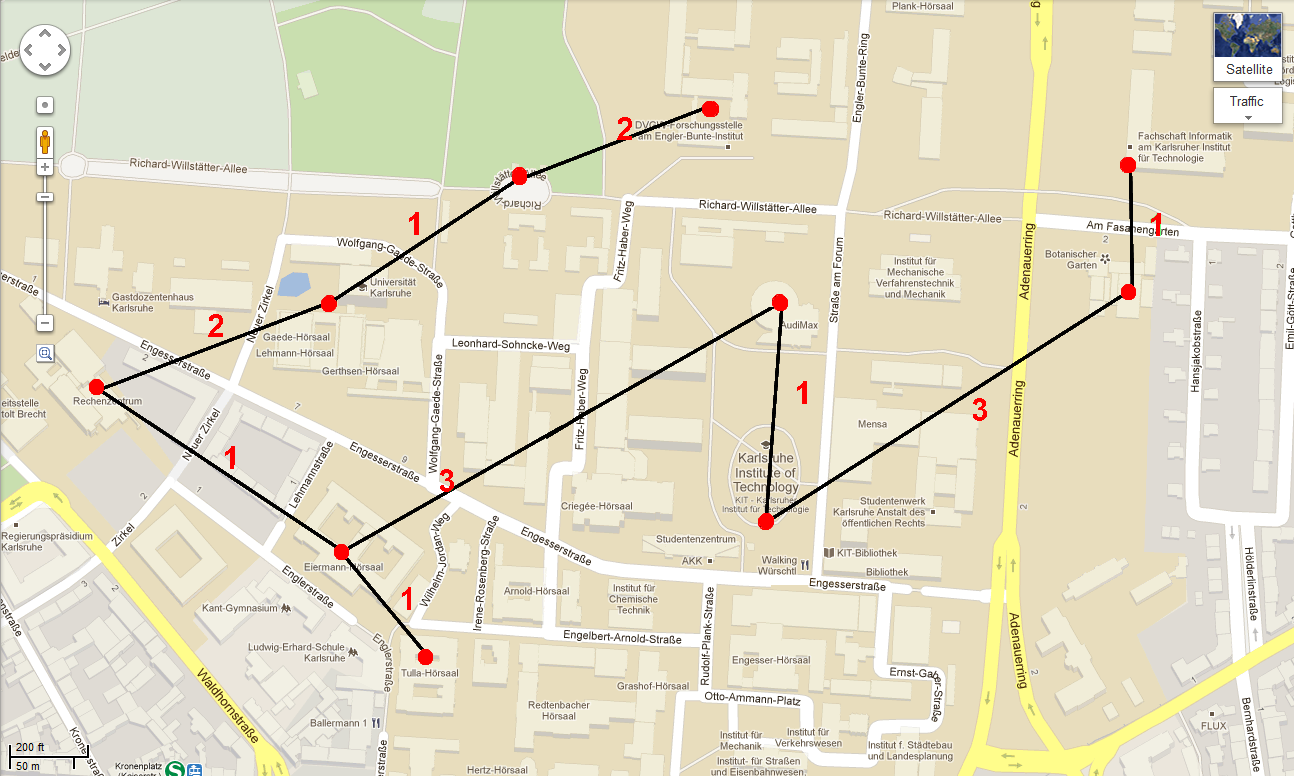
\includegraphics[scale=0.35]{Material/minSpannbaum_5.png}}
	\only<2>{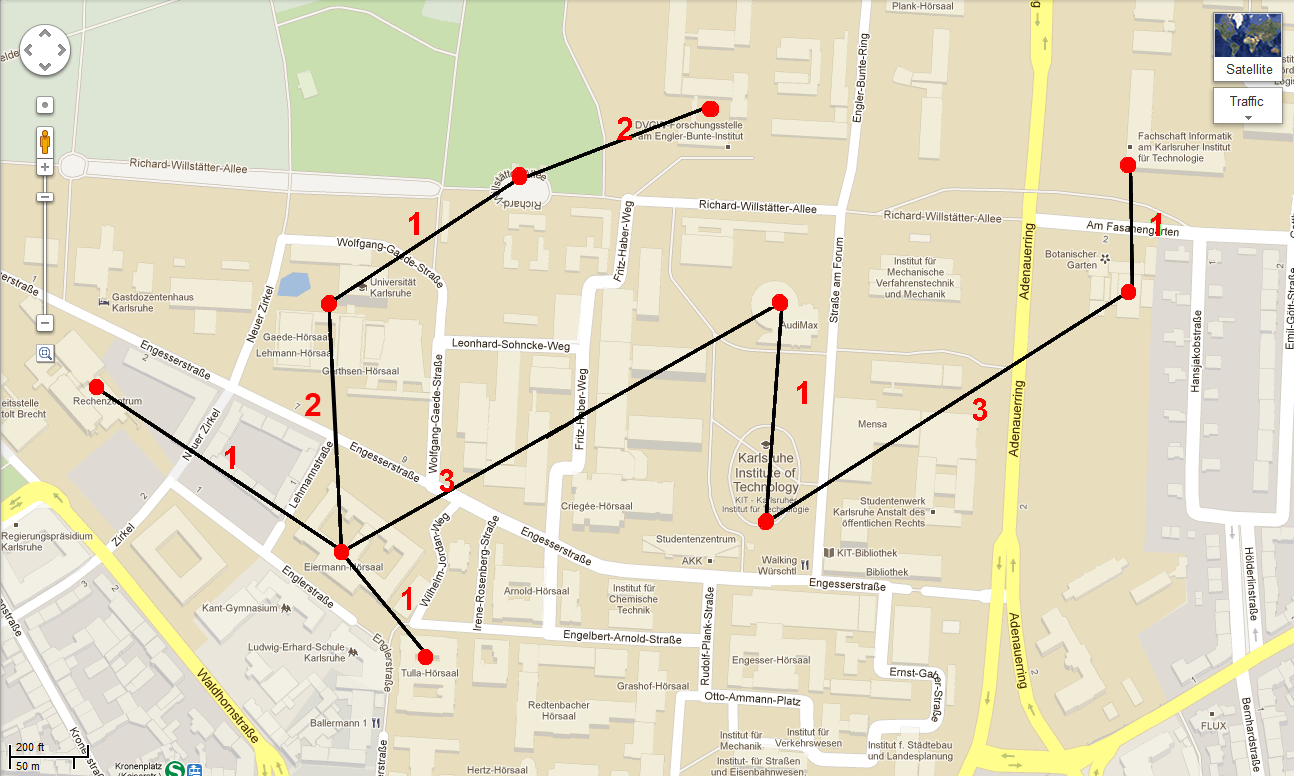
\includegraphics[scale=0.35]{Material/minSpannbaum_amb.png}}
\end{frame}

% Author: Kjell Magne Fauske
% Source: http://www.texample.net/tikz/examples/prims-algorithm/
% Declare layers
\pgfdeclarelayer{background}
\pgfsetlayers{background,main}

\subsection{Algorithmus von Prim}
\begin{frame}{Algorithmus von Prim}{Prim's algorithm}
	$S$ ist Menge aller erreichten Knoten, $E$ ist Menge der ausgewählten Kanten.\pause



	Starte bei einem beliebigen Knoten: füge zu $S$ hinzu.
	\begin{enumerate}
		\item wähle Kante am \emph{Rand} von $S$ mit dem geringsten Gewicht und füge zu $E$ hinzu. \pause
		\item füge zugehörigen Knoten zu $S$ hinzu.
		\item Fehlt ein Knoten in $S$ ? goto 1
	\end{enumerate}
\end{frame}

\begin{frame}{Algorithmus von Prim}{Prim's algorithm}
	%% Adjacency matrix of graph
	%% \  a  b  c  d  e  f  g
	%% a  x  7     5
	%% b  7  x  8  9  7
	%% c     8  x     5
	%% d  5  9     x 15  6
	%% e     7  5 15  x  8  9
	%% f           6  8  x 11
	%% g              9  11 x
	\begin{figure}
		\begin{tikzpicture}[scale=1.8, auto,swap]
			% Draw a 7,11 network
			% First we draw the vertices
			\foreach \pos/\name in {{(0,2)/a}, {(2,1)/b}, {(4,1)/c},
				                    {(0,0)/d}, {(3,0)/e}, {(2,-1)/f}, {(4,-1)/g}}
				\node[vertex] (\name) at \pos {$\name$};
			% Connect vertices with edges and draw weights
			\foreach \source/ \dest /\weight in {b/a/7, c/b/8,d/a/5,d/b/9,
				                                 e/b/7, e/c/5,e/d/15,
				                                 f/d/6,f/e/8,
				                                 g/e/9,g/f/11}
				\path[edge] (\source) -- node[weight] {$\weight$} (\dest);
			% Start animating the vertex and edge selection.
			\foreach \vertex / \fr in {d/1,a/2,f/3,b/4,e/5,c/6,g/7}
				\path<\fr-> node[selected vertex] at (\vertex) {$\vertex$};
			% For convenience we use a background layer to highlight edges
			% This way we don't have to worry about the highlighting covering
			% weight labels.
			\begin{pgfonlayer}{background}
				\pause
				\foreach \source / \dest in {d/a,d/f,a/b,b/e,e/c,e/g}
				    \path<+->[selected edge] (\source.center) -- (\dest.center);
				\foreach \source / \dest / \fr in {d/b/4,d/e/5,e/f/5,b/c/6,f/g/7}
				    \path<\fr->[ignored edge] (\source.center) -- (\dest.center);
			\end{pgfonlayer}
		\end{tikzpicture}
	\end{figure}
\end{frame}
%% end of source

\begin{frame}{Algorithmus von Prim}{Prim's algorithm}
%source http://inserv.math.muni.cz/biografie/obrazky/jarnik_vojtech.jpg
%http://www.ams.org/featurecolumn/images/january2006/trees9.jpg
	\textbf{Erfinder}
	\begin{itemize}
		\item 1930: Vojtěch Jarník
		\item 1957: Robert C. Prim
		\item 1959 wiederentdeckt von Edsger Dijkstra
	\end{itemize}

	\begin{figure}
\centering
\mbox{\subfigure{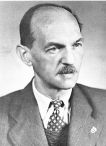
\includegraphics[width=0.6in]{Material/jarnik_vojtech.jpg}}\quad
\subfigure{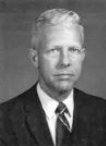
\includegraphics[width=0.6in]{Material/Prim.jpg} }}
\caption{Jarnik Vojtech und Prim}
\end{figure}
	\textbf{Alternative Bezeichnungen}
	\begin{itemize}
		\item DJP algorithm
		\item Jarník algorithm
		\item Prim–Jarník algorithm
	\end{itemize}

\end{frame}     % Algorithmus von Prim

% Author: Martin Thoma
\subsection{Algorithmus von Kruskal}
\begin{frame}{Algorithmus von Kruskal}{Kruskal's algorithm}
	$E$: Menge der ausgewählten Kanten, $S$: Menge der erreichbaren Knoten.\vspace{10pt}\pause

	So lange, bis alle Knoten erreichbar sind:

	Wähle Kante mit geringstem Gewicht

	Wenn durch ausgewählte Kante ein Knoten erreichbar ist, der davor nicht in $S$ war, füge diese Kante zu $E$ und Knoten zu $E$ hinzu.
\end{frame}


\begin{frame}{Algorithmus von Kruskal}{Kruskal's algorithm}
	\begin{figure}
		\begin{tikzpicture}[scale=1.8, auto,swap]
			% Draw a 7,11 network
			% First we draw the vertices
			\foreach \pos/\name in {{(0,2)/a}, {(2,1)/b}, {(4,1)/c},
				                    {(0,0)/d}, {(3,0)/e}, {(2,-1)/f}, {(4,-1)/g}}
				\node[vertex] (\name) at \pos {$\name$};
			% Connect vertices with edges and draw weights
			\foreach \source/ \dest /\weight in {b/a/7, c/b/8,d/a/5,d/b/9,
				                                 e/b/7, e/c/5,e/d/15,
				                                 f/d/6,f/e/8,
				                                 g/e/9,g/f/11}
				\path[edge] (\source) -- node[weight] {$\weight$} (\dest);
			% Start animating the vertex and edge selection.
			\foreach \vertex / \fr in {d/1,a/1,e/2,c/2,f/3,b/4,g/10}
				\path<\fr-> node[selected vertex] at (\vertex) {$\vertex$};
			% For convenience we use a background layer to highlight edges
			% This way we don't have to worry about the highlighting covering
			% weight labels.
			\begin{pgfonlayer}{background}
				\pause
				\foreach \source / \dest / \fr in {a/d/1,c/e/2,d/f/3,a/b/4,b/e/6,e/g/10}
				    \path<\fr->[selected edge] (\source.center) -- (\dest.center);
				\foreach \source / \dest / \fr in {d/b/5,b/c/7,d/e/8,e/f/9,f/g/11}
				    \path<\fr->[ignored edge] (\source.center) -- (\dest.center);
			\end{pgfonlayer}
		\end{tikzpicture}
	\end{figure}
\end{frame}
%% end of source

\begin{frame}[fragile]
\frametitle{Algorithmus von Kruskal}
\begin{lstlisting}
s is disjunct set of edges
n is number of edges in original graph
while s less than n - 1
e = smallest weight edge not deleted yet
    // edge e = (u, v)
    uset = s.find(u)
    vset = s.find(v)
    if (uset != vset)
        edgesAccepted = edgesAccepted + 1
        s.unionSets(uset, vset)
    end if
end while
\end{lstlisting}
\end{frame}

\begin{frame}{Algorithmus von Kruskal}{Kruskal's algorithm}
	Erfunden von:

	1956: Joseph Kruskal

	\begin{figure}
		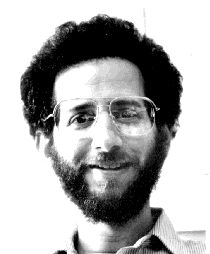
\includegraphics[scale=0.6]{Material/kruskal.jpg}
		\caption{Kruskal}
	\end{figure}
\end{frame}
  % Algorithmus von Kruskal % Minimale Spannbäume
\section{Starke Zusammenhangskomponenten}

% Martin
\subsection{Zusammenhang von Graphen: Was ist das?}
\begin{frame}{Zusammenhang von Graphen}{Connectivity}
	\begin{block}{Streng zusammenhängender Graph}
		Ein streng zusammenhängender Graph ist ein gerichteter Graph,
		in dem jeder Knoten von jedem erreichbar ist.
	\end{block}
	\begin{figure}
		\begin{tikzpicture}[->,scale=1.8, auto,swap]
			% Draw a 7,11 network
			% First we draw the vertices
			\foreach \pos/\name in {{(0,0)/a}, {(0,2)/b}, {(1,2)/c},
				                    {(1,0)/d}, {(2,1)/e}, {(3,1)/f},
									{(3,2)/g}, {(2,0)/h}}
				\node[vertex] (\name) at \pos {$\name$};
			% Connect vertices with edges and draw weights
			\foreach \source/ \dest /\pos in {a/b/,b/c/,c/d/,d/a/,
										c/e/bend left, d/e/,e/c/, f/g/,
										g/f/bend left, d/h/}
				\path (\source) edge [\pos] node {} (\dest);
		\end{tikzpicture}
	\end{figure}
\end{frame}

\begin{frame}{Zusammenhang von Graphen}{Connectivity}
	\begin{block}{Zusammenhangskomponente}
		Eine Zusammenhangskomponente ist ein maximaler Subgraph S
		eines gerichteten Graphen, wobei S streng zusammenhängend ist.
		% Muss dieser Subgraph maximal sein?
	\end{block}
	\begin{figure}
		\begin{tikzpicture}[->,scale=1.8, auto,swap]
			% Draw a 7,11 network
			% First we draw the vertices
			\foreach \pos/\name in {{(0,0)/a}, {(0,2)/b}, {(1,2)/c},
				                    {(1,0)/d}, {(2,1)/e}, {(3,1)/f},
									{(3,2)/g}, {(2,0)/h}}
				\node[vertex] (\name) at \pos {$\name$};
			% Connect vertices with edges
			\foreach \source/ \dest /\pos in {a/b/,b/c/,c/d/,d/a/,
										c/e/bend left, d/e/,e/c/, f/g/,
										g/f/bend left, d/h/}
				\path (\source) edge [\pos] node {} (\dest);

			% colorize the vertices
			\foreach \vertex in {a,b,c,d,e}
				\path node[selected vertex] at (\vertex) {$\vertex$};

			\foreach \vertex in {f,g}
				\path node[blue vertex] at (\vertex) {$\vertex$};

			\foreach \vertex in {h}
				\path node[yellow vertex] at (\vertex) {$\vertex$};
		\end{tikzpicture}
	\end{figure}
\end{frame}

\begin{frame}{Elementare Eigenschaften}
	\begin{block}{}
		    Die Knotenmengen verschiedener SCCs sind disjunkt.
	\end{block}

	\begin{block}{}
		    SCCs bilden Zyklen.
	\end{block}

	\begin{block}{}
		    Die Vereinigung aller Knoten aller SCCs ergibt alle Knoten
			des ursprünglichen Graphen.
	\end{block}
\end{frame}
 % Zusammenhängende Graphen allgemein erklärt
\subsection{SCCs finden}
\begin{frame}{Wie findet man SCCs?}{}
\begin{wrapfigure}{r}{150px}
  \begin{center}
    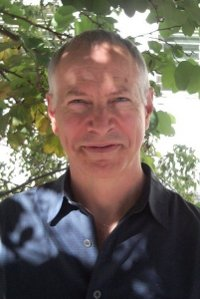
\includegraphics{Material/Bob_Tarjan.jpg}
  \end{center}
  \caption{Robert Tarjan}
\end{wrapfigure}
Algorithmus von Robert Tarjan

% Source: http://commons.wikimedia.org/wiki/File:Bob_Tarjan.jpg

nutzt Tiefensuche im Graphen
\end{frame}


\tikzstyle StackBox=[style=help lines,color=blue!50,fill=white]
\tikzstyle{abstract}=[rectangle, draw=black,
		fill=orange!40,
        text centered, anchor=center, text=white, text width=0.4cm, text height=0.4cm]
\tikzstyle{textstyle}=[rectangle, draw=white,
		fill=white, anchor=base west, text=black, text width=3cm, text height=0.4cm]
\tikzstyle{textstyleMini}=[rectangle, draw=white,
		fill=white, anchor=center, text=black, text width=0.5cm, text height=0.4cm]

\begin{frame}

\begin{algorithm}[H]
	\begin{algorithmic}
		\Function{startTarjan}{Graph g}
			\State $indexCounter \gets 0$
			\State $stack$
			\ForAll{$node$ in $g$}
				\If{$!node.visited$}
					\Call{tarjan}{$node$}
				\EndIf
			\EndFor
		\EndFunction
	\end{algorithmic}
\caption{Tarjans Algorithmus zur bestimmung starker Zusammenhangskomponenten}
\label{alg:seq1}
\end{algorithm}
\end{frame}

\begin{frame}
\begin{algorithm}[H]
    \begin{algorithmic}
        \Function{tarjan}{Node* node}
            \State $node.visited \gets $ \textbf{true}
            \State $node.index \gets indexCounter++$
            \State $stack.push(node)$
            \ForAll{$successor$ in $node.successors$}
                \If{$!node.visited$}
                    \Call{tarjan}{successor}
                \EndIf
                \State $node.lowlink \gets$ \Call{min}{$node.lowlink, successor.lowlink$}
            \EndFor

            \boxto<1->{a}\If{$node.lowlink == node.index$}
                \Repeat
                    \State $successor \gets stack.pop()$
                \Until{$successor == node$}
            \EndIf\tikzmark{a}
        \EndFunction
    \end{algorithmic}
\label{alg:seq2}
\end{algorithm}

% To insert the annotation
\begin{tikzpicture}[remember picture,overlay]
\coordinate (a) at ($(a)+(8.5,3)$); % <= adjust this parameter to move the position of the annotation
\node[rectangle,draw, gray,text width=3cm,align=left,right] at (a) {SCC wurde gefunden, ggf. ausgeben};
\end{tikzpicture}
\end{frame}

\begin{frame}{Wie findet man SCCs?}{}
	\begin{figure}
		\begin{tikzpicture}[->,scale=1.8, auto,swap]
			\node[textstyle] (Text) at (0,3) {Rekursionstiefe:};
			\node[textstyle] (RecDepth) at (3,3) {};

			% Draw the vertices
			\foreach \pos/\name in {{(0,0)/a}, {(0,2)/b}, {(1,2)/c},
				                    {(1,0)/d}, {(2,1)/e}, {(3,1)/f},
									{(4,2)/g}, {(5,2)/h}, {(4,0)/i},
									{(5,0)/j}}
				\node[vertex] (\name) at \pos {$\name$};

			% Connect vertices with edges
			\foreach \source/ \dest /\pos in {a/b/,b/c/,c/d/,d/a/,
										c/e/bend left, d/e/,e/c/,
										e/f/,
										f/g/, f/i/,g/f/bend right,i/f/bend left,
										g/h/, h/j/, j/i/, i/g/}
				\path (\source) edge [\pos] node {} (\dest);

			% Start animating the vertex and edge selection.
			\foreach \vertex / \fr / \lowlink / \index in {a/1/0/0,b/2/1/1,c/3/2/2,d/4/0/3,e/5/2/4,f/6/5/5,g/7/6/6,h/8/7/7,j/9/8/8,i/10/5/9} {
				\path<\fr-> node[selected vertex] at (\vertex) {$\vertex_{\lowlink, \index}$};
				\path<\fr-> node[textstyleMini] at (RecDepth) {$\index$};
			}
			% Start animating the edge selection.
			% For convenience we use a background layer to highlight edges
			% This way we don't have to worry about the highlighting covering
			% weight labels.
			\begin{pgfonlayer}{background}
				    \path<4->[ignored edge] (d.center) edge [] node {} (a.center);
				    \path<5->[ignored edge] (e.center) edge [] node {} (c.center);
				    \path<10->[ignored edge] (i.center) edge [bend left] node {} (f.center);
				\foreach \source / \dest / \fr / \pos in {a/b/2/,b/c/3/,c/d/4/, d/e/5/,e/f/6/,f/g/7/,g/h/8/,
														h/j/9/,j/i/10/}
				    \path<\fr->[selected edge] (\source.center) edge [\pos] node {} (\dest.center);
			\end{pgfonlayer}
			% go back in recursion
			% Start animating.
			\foreach \vertex / \fr / \lowlink / \index in {j/11/5/8,h/12/5/7,g/13/5/6,f/14/5/5} {
				\path<\fr-> node[selected vertex] at (\vertex) {$\vertex_{\lowlink, \index}$};
				\path<\fr-> node[textstyleMini] at (RecDepth) {$\index$};
			}
			% mark first scc
			\begin{pgfonlayer}{background}
				\path<15->[color=blue,fill=green!20] (4.2,1) circle (1.6cm);
			\end{pgfonlayer}
			% go back in recursion
			% Start animating.
			\foreach \vertex / \fr / \lowlink / \index in {e/16/2/4,c/17/0/3,b/18/0/1,a/19/0/0} {
				\path<\fr-> node[selected vertex] at (\vertex) {$\vertex_{\lowlink, \index}$};
				\path<\fr-> node[textstyleMini] at (RecDepth) {$\index$};
			}
			% mark first scc
			\begin{pgfonlayer}{background}
				\path<20->[color=blue,fill=green!20] (0.6,1) circle (1.6cm);
			\end{pgfonlayer}
		\end{tikzpicture}
	\end{figure}
\end{frame}
   % Wie findet man SCCs?
\begin{frame}
\begin{block}{}
        Gibt es noch Fragen zum finden von SCCs?
\end{block}
\end{frame}
       % Gibt es noch Fragen?


% Max:
\subsection{Brücke}
\begin{frame}{Brücke}{Bridge}
	\begin{block}{Definition: Brücke}
		Eine Kante $e \in E$ eines Graphen $G(V,E)$ heißt Brücke \\
		$: \Leftrightarrow$ Durch das Entfernen von e zerfällt G in mehr zusammenhängende Teilgraphen,
		als G bereits hat. \\
		$: \Leftrightarrow$ Sie ist in keinem Zyklus enthalten
	\end{block}

	\begin{figure}
		\begin{tikzpicture}[scale=1.8, auto,swap]
			% Draw a 7,11 network
			% First we draw the vertices
			\foreach \pos/\name in {{(0,0)/a}, {(0,2)/b}, {(1,2)/c},
				                    {(1,0)/d}, {(2,1)/e}, {(3,1)/f},
									{(4,2)/g}, {(5,2)/h}, {(4,0)/i},
									{(5,0)/j}}
				\node[vertex] (\name) at \pos {$\name$};
			% Connect vertices with edges
			\foreach \source/ \dest /\pos in {a/b/,b/c/,c/d/,d/a/,
										d/e/,e/c/,
										e/f/,
										f/g/, f/i/,
										g/h/, h/j/, j/i/, i/g/}
				\path (\source) edge [\pos] node {} (\dest);
			\begin{pgfonlayer}{background} \path<+->[selected edge] (e.center) -- (f.center); \end{pgfonlayer}
		\end{tikzpicture}
	\end{figure}
\end{frame}

\begin{frame}
	\frametitle{Wozu?}
	\begin{itemize}
		\item Relevanz: Brücken und Artikulationspunkte (später) sind Teile des Graphen, die für die Kommunikation im Graphen unabdingbar sind. \\
	\end{itemize}
	Wir wollen Artikulationspunkte und Brücken auch algorithmisch finden. \\ $\Rightarrow$ Lösung: Tiefensuche \\
	\pause
	Komplexität: $\mathcal{O}(|V| + |E|)$
\end{frame}

\begin{frame}
	\frametitle{Wie findet man Brücken?}
	\begin{itemize}
		\item Algorithmus von Tarjan in $\mathcal{O}(|V| + |E|)$
		\item Zweiter, tollerer Algorithmus:
			\begin{itemize}
				\item Gehe mit Tiefensuche durch Graph, nummeriere Knoten $v \in V$ mit $N(v)$
				\item Merke für jeden Knoten $v \in V$ folgendes $L(v)$:\\
					% Oh how passionately I hate latex.
					 $ L(v) := \min\{ N(c) $ ~\\ $ \mid c \in V \wedge \text{c erreichbar von v durch max. eine Rückwärtskante} \} $
				\item Baumkante $(p,c) \in E$  mit $p,c \in V$ ist nun Brücke gdw. $L(c) > N(p)$
			\end{itemize}
	\end{itemize}
%	<Tafelbeispiel>

\end{frame}

                    % Brücke
\subsection{Artikulationspunkt}
\begin{frame}{Artikulationspunkt}{Articulation vertex or cut vertices}
	\begin{block}{Definition: Artikulationspunkt (auch "Gelenkpunkt" genannt)}
		Ein Knoten $v \in V$ eines Graphen $G(V,E)$ heißt Artikulationspunkt
		$: \Leftrightarrow$ Durch das Entfernen von v zerfällt G in mehr zusammenhängende Teilgraphen,
		als G bereits hat.
	\end{block}
	\begin{figure}
		\begin{tikzpicture}[scale=1.8, auto,swap]
			% Draw a 7,11 network
			% First we draw the vertices
			\foreach \pos/\name in {{(0,0)/a}, {(1,0)/b}, {(2,0)/c},
									{(3,0)/d}, {(2.5,0.7)/e}}
				\node[vertex] (\name) at \pos {$\name$};
			% Connect vertices with edges and draw weights
			\foreach \source/ \dest /\pos in {a/b/,b/c/,c/d/,c/e/,d/e/}
				\path (\source) edge [\pos] node {} (\dest);
		\end{tikzpicture}
	\end{figure}
\end{frame}


\begin{frame}
	\frametitle{Algorithmus}
	Fast wie für Brücken. Unterschiede:
	\begin{itemize}
		\item $L(v)$ hier anders definiert: bei Rückwärtskanten erst nach mindestens einer Baumkante
		\item Hier vergleichen wir für alle $v \in V$ $L(v)$ und $N(v)$: \\
	$v$ ist Art.-punkt $\Leftrightarrow L(v) = N(v)$
	\end{itemize}
	\begin{figure}
		\begin{tikzpicture}[scale=1.8, auto,swap]
			% Draw a 7,11 network
			% First we draw the vertices
			\foreach \pos/\name in {{(0,0)/a}, {(1,0)/b}, {(2,0)/c},
									{(3,0)/d}, {(2.5,0.7)/e}}
				\node[vertex] (\name) at \pos {$\name$};
			% Connect vertices with edges and draw weights
			\foreach \source/ \dest /\pos in {a/b/,b/c/,c/d/,c/e/,d/e/}
				\path (\source) edge [\pos] node {} (\dest);
		\end{tikzpicture}
	\end{figure}
%	\begin{figure}
%		\begin{tikzpicture}[scale=1.8, auto, swap]
%			\foreach \pos/\name in {{(0.5,1.5)/e}, {(1,1)/c}, {(1.5,0.5)/d}, {(0.5,0.5)/b}, {(0,0)/a}}
%				\node[vertex] (\name) at \pos {$\name$};
%			% Connect vertices with edges and draw weights
%			\foreach \source/ \dest /\pos in {a/b/,b/c/,d/c/,e/c/,d/e/}
%				\path (\source) edge [\pos] node {} (\dest);
%		\end{tikzpicture}
%	\end{figure}
%	<Beispiel eines Algorithmus-Durchlaufs>
\end{frame}
        % Artikulationspunkt
\subsection{Zweifachverbundener Graph}
\begin{frame}{Zweifachverbundener Graph}{Biconnected graph}
	\begin{block}{Zweifachverbundener Graph}
		Ein Graph $G=(E,V)$ ist genau dann zweifach verbunden (engl. biconnected), wenn er keine Artikulationspunkte enthält.
	\end{block}
	Problem: Ist gegebener Graph zweifach verbunden? \\
	$\Rightarrow$ Suche nach Artikulationspunken!
\end{frame}

\begin{frame}{Beispiel}
	\begin{figure}
		\begin{tikzpicture}[scale=1.8, auto,swap]
			% Draw a 7,11 network
			% First we draw the vertices
			\foreach \pos/\name in {{(0,0)/a}, {(0,2)/b}, {(1,2)/c},
				                    {(1,0)/d}, {(2,1)/e}, {(3,1)/f},
									{(4,2)/g}, {(5,2)/h}, {(4,0)/i},
									{(5,0)/j}}
				\node[vertex] (\name) at \pos {$\name$};
			% Connect vertices with edges
			\foreach \source/ \dest /\pos in {a/b/,b/c/,c/d/,d/a/,
										d/e/,e/c/,
										e/f/,
										f/g/, f/i/,g/c/,
										g/h/, h/j/, j/i/, i/g/}
				\path (\source) edge [\pos] node {} (\dest);
		\end{tikzpicture}
	\end{figure}
\end{frame}
 % Zweifachverbundener-Graph
                % Starke zusammenhangskomponenten
\section{Färbung von Graphen}
\subsection{}
\begin{frame}{Färbung von Graphen}{Graph coloring}
	\begin{block}{Problem COLOR}
		Gegeben sei ein Graph $G = (V, E)$ und ein Parameter $K \in \mathbb{N}$.
		Frage: Gibt es eine Knotenfärbung von $G$ mit höchstens $K$ Farben,
		so dass je zwei adjazente Knoten verschiedene Farben besitzen?
	\end{block}
	\begin{itemize}
		\item Ist für 2 Farben entscheidbar (bipartite Graphen)
		\item Für 3 Farben schon $\mathcal{NP}$-vollständig \\
			(Sogar $\mathcal{NP}$-schwer einen 3-färbbaren Graphen mit 4 Farben zu färben)
		\item Für 4 Farben für planare Graphen bewiesenermaßen immer möglich
	\end{itemize}
\end{frame}

\begin{frame}{2-COLOR}{Bipartite Graphen}
	Problem: Gegeben Graph $G=(V, E)$. Ist dieser eine Ja-Instanz von 2-COLOR?

	Lösungsansatz:
	\begin{itemize}
		\item Tiefensuche
		\item Wechsle Farbe nach jedem Knoten
		\item Bei Konflikten breche ab und antworte "Nein"
	\end{itemize}
	Läuft die Tiefensuche ohne abzubrechen durch, ist der Graph bipartit. Aus dem Algorithmus folgt bereits eine gültige Färbung.
\end{frame}

\begin{frame}{3-COLOR}
	Auch hier: Ist Graph $G = (V,E)$ mit 3 Farben färbbar? \\
	Achtung: Problem ist $\mathcal{NP}$-Vollständig.
	\\
	Das heißt es ist kein effizienter Algorithmus bekannt, Laufzeit zur Lösung steigt i.A. exponentiell. \\
	Brute-force für kleine Instanzen des Problems praktikabel. \\
	Für größere Instanzen bietet sich Transformation zu $\mathcal{SAT}$ und Lösung per SAT-Solver an.

\end{frame}
      % Färbung von Graphen
\section{Kreise}

\subsection{Eulerkreisproblem}

\begin{frame}{Eulerkreisproblem}{Eulerian path}
	\begin{block}{Erklärung}
		Ein Eulerkreis ist ein Kreis in einem Graphen, in dem jede Kante genau einmal benutzt wird.
	\end{block}
\end{frame}

\begin{frame}{Eulerkreisproblem}{Bedingungen}
	\begin{block}{Im ungerichteten Graph}
		Es existiert ein Eulerkreis\\
		$\Leftrightarrow$ Der Graph ist zusammenhängend und jeder Knoten hat geraden Grad
	\end{block}

	\begin{block}{Im gerichteten Graph}
		Es existiert ein Eulerkreis\\
		$\Leftrightarrow$ Der Graph ist stark zusammenhängend und für jeden Knoten gilt: Eingangsgrad = Ausgangsgrad
	\end{block}
\end{frame}

\begin{frame}{Algorithmus von Fleury}
	Das Eulerkreisproblem ist effizient lösbar:

	Algorithmus von Fleury $\in {\cal O}(|E|^2) $:

	\begin{enumerate}
		\item Start bei einem beliebigen Knoten
		\item Wähle eine unmarkierte von dem Knoten ausgehende Kante, die wenn möglich im Restgraphen keine Brückenkante ist. Wenn es nur Brückenkanten gibt, dann dann wird die Kante zu dem Knoten genommen, der den höhere Ausgangsgrad hat
		\item Markiere diese Kante, füge sie der Kreis hinzu
		\item Wähle den zu der markierten Kante adjazenten Knoten
		\item Wenn dieser Knoten noch unmarkierte Kanten besitzt: \\GOTO 2.
	\end{enumerate}
\end{frame}

%\begin{frame}{Algorithmus von Fleury}{Anwendungsbeispiel}
%	Wortmenge: $\{$as, man, meet, nets, set, sum, tea, team$\}$
%
%	Menge der Anfangs- und Endbuchstaben: $\{$a, m, n, s, t$\}$
%	\begin{figure}
%		\begin{tikzpicture}[->,scale=1.8, auto,swap]
%			% Draw a 7,11 network
%			% First we draw the vertices
%			\foreach \pos/\name in {{(0,0)/a}, {(0,2)/s},
%				                    {(4,0)/m}, {(2,2)/t}, {(3,2)/n}}
%				\node[vertex] (\name) at \pos {$\name$};
%			% Connect vertices with edges and draw weights
%			\foreach \source/ \dest /\foo /\pos in {a/s/as/,s/m/sum/bend right,
%										s/t/set/, m/t/meet/bend left,m/n/man/bend right,
%										t/a/tea/bend left, t/m/team/bend left, n/s/nets/bend right}
%				\path (\source) edge [\pos] node {\foo} (\dest);
%		\end{tikzpicture}
%	\end{figure}
%\end{frame}

\begin{frame}{Algorithmus von Fleury}{Anwendungsbeispiel}
	\begin{figure}
		\begin{tikzpicture}[->,scale=1.7, auto,swap]
			% Draw a 7,11 network
			% First we draw the vertices
			\foreach \pos/\name in {{(0,1)/a}, {(2,0)/c}, {(2,3)/b},
									{(4,3)/d}, {(4,1)/e}, {(6,2)/f}, {(6,0)/g}}
				\node[vertex] (\name) at \pos {$\name$};
			% Connect vertices with edges and draw weights
			\foreach \source/ \dest /\pos in {b/a/,c/a/,a/d/,a/e/,c/b/, d/b/, b/e/, e/c/, g/c/, e/d/, d/f/, f/g/}
				\path (\source) edge [\pos] node {} (\dest);
			% Start animating the edge selection.
			% For convenience we use a background layer to highlight edges
			% This way we don't have to worry about the highlighting covering
			% weight labels.
			\begin{pgfonlayer}{background}
				\foreach \source / \dest / \fr / \pos in {a/a/1/, a/e/2/, e/d/3/, d/b/4/, b/a/5/,
														a/d/6/, d/f/7/, f/g/8/, g/c/9/, c/b/10/,
														b/e/11/, e/c/12/, c/a/13/}
				    \path<\fr->[selected edge] (\source.center) edge [\pos] node {} (\dest.center);
			\end{pgfonlayer}
		\end{tikzpicture}
	\end{figure}
\end{frame}

\begin{frame}{Algorithmus von Hierholz}
	Effizienter als Fleury

	\begin{enumerate}
		\item Start bei einem beliebigen Knoten v
		\item Folge so lange Kanten, bis man wieder in v ist
		\item Wiederhole diesen Schritt bei einem Knoten, der bereits in einem Kreis ist und der noch unmarkierte Kanten hat
	\end{enumerate}
\end{frame}

\begin{frame}{Algorithmus von Hierholz}{Anwendungsbeispiel}
	\begin{figure}
		\begin{tikzpicture}[->,scale=1.7, auto,swap]
			% Draw a 7,11 network
			% First we draw the vertices
			\foreach \pos/\name in {{(0,1)/a}, {(2,0)/c}, {(2,3)/b},
									{(4,3)/d}, {(4,1)/e}, {(6,2)/f}, {(6,0)/g}}
				\node[vertex] (\name) at \pos {$\name$};
			% Connect vertices with edges and draw weights
			\foreach \source/ \dest /\pos in {b/a/,c/a/,a/d/,a/e/,c/b/, d/b/, b/e/, e/c/, g/c/, e/d/, d/f/, f/g/}
				\path (\source) edge [\pos] node {} (\dest);
			% Start animating the edge selection.
			% For convenience we use a background layer to highlight edges
			% This way we don't have to worry about the highlighting covering
			% weight labels.
			\begin{pgfonlayer}{background}
				\foreach \source / \dest / \fr / \pos in {a/a/1/, a/e/2/, e/d/3/, d/b/4/, b/a/5/,
														e/c/6/, c/b/7/, b/e/8/, d/f/9/, f/g/10/,
														g/c/11/, c/a/12/, a/d/13/}
				    \path<\fr->[selected edge] (\source.center) edge [\pos] node {} (\dest.center);
			\end{pgfonlayer}
		\end{tikzpicture}
	\end{figure}
\end{frame}

\begin{frame}{Eulerpfad}
	\begin{figure}
		\begin{tikzpicture}[,scale=1.8, auto,swap]
			% Draw a 7,11 network
			% First we draw the vertices
			\foreach \pos/\name in {{(0,0)/a}, {(2,0)/b}, {(0,2)/c},
				                    {(2,2)/d}, {(1,3)/e}}
				\node[vertex] (\name) at \pos {$\name$};
			% Connect vertices with edges and draw weights
			\foreach \source/ \dest /\pos in {a/b/,b/c/, c/d/, d/e/, a/c/, a/d/, b/d/, c/e/}
				\path (\source) edge [\pos] node {} (\dest);
			% Start animating the edge selection.
						% For convenience we use a background layer to highlight edges
			% This way we don't have to worry about the highlighting covering
			% weight labels.
			\begin{pgfonlayer}{background}
				\foreach \source / \dest / \fr / \pos in {a/a/1/, b/d/2/, d/c/3/, c/e/4/, e/d/5/, d/a/6/,
														a/b/7/, b/c/8/, c/a/9/}
				    \path<\fr->[selected edge] (\source.center) edge [\pos] node {} (\dest.center);
			\end{pgfonlayer}
		\end{tikzpicture}
	\end{figure}
	Es kann einen Eulerpfad, aber keinen Eulerkreis geben
\end{frame}        % Eulerkreisproblem
\subsection{Hamiltonkreisproblem}

\begin{frame}{Hamiltonkreisproblem}{Hamiltonian path}
	\begin{block}{Erklärung}
		Ein Hamiltonkreis ist ein Kreis in einem Graphen, in dem jeder Knoten genau einmal benutzt wird.\\

		Das Hamiltonkreisproblem ist NP-vollständig.
	\end{block}
\end{frame}

\begin{frame}{Hamiltonkreisproblem}{Bedingungen und Kriterien (Auszug)}
	\begin{block}{Kriterien (notwendig)}
		\begin{itemize}
			\item G hat keine Schnittknoten
			\item G hat keine Brückenkanten
			\item G hat Minimalgrad $\geq 2$
		\end{itemize}
	\end{block}
	\begin{block}{Bedingungen}
		Bei Graphen G mit $n \geq 3$ Knoten
		\begin{itemize}
			\item G hat Minimalgrad $\frac{n}{2} \Rightarrow$ $\exists $ Hamiltonkreis
			\item G ist vollständig $\Rightarrow \exists$ Hamiltonkreis
			\item G ist Kantengraph eines eulerschen oder hamiltonschen Graphen
		\end{itemize}
	\end{block}
\end{frame}

\begin{frame}{Hamilton- und Eulerkreisproblem}{Anwendungsbeispiel}
	\begin{block}{Gegeben}
		Eine Menge von Wörtern
	\end{block}
	\begin{block}{Gesucht}
		Aneinanderreihung von Wörtern, sodass jeweils Anfangs- und Endbuchstaben gleich sind
		(auch im Ringschluss).
	\end{block}
\end{frame}


\begin{frame}{Hamilton- und Eulerkreisproblem}{Anwendungsbeispiel}
	Wortmenge: $\{$as, man, meet, nets, set, sum, tea, team$\}$

	Menge der Anfangs- und Endbuchstaben: $\{$a, m, n, s, t$\}$
	\begin{figure}
		\begin{tikzpicture}[->,scale=1.3, auto,swap]
			% First we draw the vertices
			\foreach \pos/\name in {{(1,0)/nets}, {(3,0)/set}, {(5,0)/tea},
				                    {(0,2)/man}, {(6,2)/team}, {(1,4)/as},
									{(3,4)/sum}, {(5,4)/meet}}
				\node[vertex] (\name) at \pos {$\name$};
			% Connect vertices with edges and draw weights
			\foreach \source/ \dest /\pos in {nets/set/, nets/sum/, set/tea/, set/team/,
									tea/as/, man/nets/, team/man/, team/meet/, as/set/,
									as/sum/, sum/meet/, sum/man/, meet/team/bend left, meet/tea/}
				\path (\source) edge [\pos] node {} (\dest);
			% Start animating the edge selection.
			% For convenience we use a background layer to highlight edges
			% This way we don't have to worry about the highlighting covering
			% weight labels.
			\begin{pgfonlayer}{background}
				\foreach \source / \dest / \fr / \pos in { as/as/1/, as/sum/2/, sum/man/3/, man/nets/4/,
									nets/set/5/, set/team/6/, team/meet/7/, meet/tea/8/, tea/as/9/}
				    \path<\fr->[selected edge] (\source.center) edge [\pos] node {} (\dest.center);
			\end{pgfonlayer}
		\end{tikzpicture}
	\end{figure}
%		Animierter Graph mit einem Hamiltonkreis. (ohne speziellen Algorithmus?) Wie ausführlich sollen Hamiltonkreise noch genau behandelt werden?
\end{frame}


\begin{frame}{Hamilton- und Eulerkreisproblem}{Anwendungsbeispiel}
	Wortmenge: $\{$as, man, meet, nets, set, sum, tea, team$\}$

	Menge der Anfangs- und Endbuchstaben: $\{$a, m, n, s, t$\}$
	\begin{figure}
		\begin{tikzpicture}[->,scale=1.8, auto,swap]
			% Draw a 7,11 network
			% First we draw the vertices
			\foreach \pos/\name in {{(0,0)/a}, {(0,2)/s},
				                    {(4,0)/m}, {(2,2)/t}, {(3,2)/n}}
				\node[vertex] (\name) at \pos {$\name$};
			% Connect vertices with edges and draw weights
			\tikzstyle{LabelStyle}=[fill=white, fill opacity=0.0, text opacity=1,sloped]
			\foreach \source/ \dest /\foo /\pos in {a/s/as/,s/m/sum/bend right,
										s/t/set/, m/t/meet/bend left,m/n/man/bend right,
										t/a/tea/bend left, t/m/team/bend left, n/s/nets/bend right}
				%\path (\source) edge [\pos] node {\foo} (\dest);
				\Edge[label=\foo,style={\pos}](\source)(\dest);
			% Start animating the edge selection.
			% For convenience we use a background layer to highlight edges
			% This way we don't have to worry about the highlighting covering
			% weight labels.
			\begin{pgfonlayer}{background}
				\foreach \source / \dest / \fr / \pos in {s/s/1/, s/t/2/, t/m/3/bend left, m/n/4/bend right, n/s/5/bend right,
														s/m/6/bend right, m/t/7/bend left, t/a/8/bend left, a/s/9/}
				    \path<\fr->[selected edge] (\source.center) edge [\pos] node {} (\dest.center);
			\end{pgfonlayer}
		\end{tikzpicture}
	\end{figure}
\end{frame}
     % Hamiltonkreisproblem
             % Euler- und Hamilton-Kreise

\section{Abspann}
\subsection{Abspann}

\begin{frame}{}
Vielen Dank für eure Aufmerksamkeit!
\end{frame}
\begin{frame}{Literatur}
  \begin{itemize}
  \item SCC: Introduction to Algorithms. Second Edition. Thomas H. Cormen. S. 552 - 560.
  \item Minimum Spanning Trees: Introduction to Algorithms. Second Edition. Thomas H. Cormen. S. 561 - 579.
  \item Hamiltonian-cycle problem: Introduction to Algorithms. Second Edition. Thomas H. Cormen. S. 1008 - 1013.
  \item Euler tour: Introduction to Algorithms. Second Edition. Thomas H. Cormen. S. 966.
  \end{itemize}
\end{frame}
          % Quellen und weitere Infos
\begin{frame}{Quellen}
	Quelltext dieser Präsentation auf \href{https://github.com/MartinThoma/ICPC-Referat}{GitHub}

	\textbf{Bilder}
	\begin{itemize}
		\item Jarnik Vojtech:\url{http://inserv.math.muni.cz/biografie/obrazky/jarnik_vojtech.jpg}
		\item Prim: \url{http://www.ams.org/featurecolumn/images/january2006/trees9.jpg}
		\item Kruskal: \url{http://www.cs.umd.edu/~kruskal/kruskal.gif}
		\item Tarjan: \url{http://commons.wikimedia.org/wiki/File:Bob_Tarjan.jpg}
	\end{itemize}

 	\textbf{Tkiz Source}
 	\begin{itemize}
 		\item Prim: \url{http://www.texample.net/tikz/examples/prims-algorithm/}
 	\end{itemize}
\end{frame}


\end{document}
